\documentclass[10pt, journal]{IEEEtran}

\usepackage[utf8]{inputenc}
\usepackage[T1]{fontenc}
\usepackage[english]{babel}
\usepackage{lmodern}
\usepackage{microtype}
\usepackage{amsmath, amssymb, amsthm, mathtools, bm}
\newtheorem{lemma}{Lemma}
\newtheorem{theorem}{Theorem}
\newtheorem{proposition}{Proposition}
\usepackage{siunitx}
\sisetup{locale = US, detect-all = true, exponent-product = \cdot}
\usepackage{booktabs, array, tabularx, multirow, makecell, colortbl}
\usepackage{graphicx}
\graphicspath{{figuras/}}
\usepackage{tikz}
\usetikzlibrary{arrows.meta, positioning, calc, shapes.geometric}
\usepackage{algorithm}
\usepackage{algpseudocode}
\usepackage{cite}
\usepackage{hyperref}
\hypersetup{colorlinks=true, linkcolor=blue, citecolor=blue, urlcolor=blue}

%% --- Paleta cromática institucional SENI-IA ---
\definecolor{seni-blue}{RGB}{0,45,98}
\definecolor{seni-red}{RGB}{206,17,38}
\definecolor{seni-gold}{RGB}{201,168,76}
\definecolor{seni-green}{RGB}{0,122,51}
\definecolor{seni-dark}{RGB}{26,26,26}

%% ====================================================================
%% CUADRO DE TÍTULOS SOBERANOS (4 OPCIONES CANÓNICAS EN PORTADA)
\title{SENI-142: An Open-Access Resilient Insular Transmission Benchmark of the Dominican Republic with Diakoptic Territorial Decomposition under Spatial Planning Law 368-22 --- Part~2: Multi-Vector Flexibility, Scalable Silicon Campaign, and Operational Telemetry}
\author{Junior~Alexis~Villanueva-Rosario,~\IEEEmembership{Ms.C., Ph.D.(c)}\\[0.3em]
{\normalsize\textnormal{\textbf{V-TECH} \textbar\ \textbf{V-CORE TECH S.R.L.} / \textbf{Villa-Core Technologies, S.L.}}}\\[0.15em]
{\footnotesize\textnormal{\textit{Department of Electrical Grids and Renewable Energy (EERR) Research}}}\\[0.15em]
{\footnotesize\textnormal{\textit{Doctoral Chair in Power Systems and Artificial Intelligence}}}\\[0.15em]
{\footnotesize\textnormal{Santo Domingo, Dominican Republic \textbar\ \texttt{ingjavillanueva@gmail.com}}}%
\thanks{J. A. Villanueva-Rosario is with the Department of Electrical Grids and Renewable Energy (EERR) Research, V-TECH (V-CORE TECH S.R.L. / Villa-Core Technologies, S.L.), Santo Domingo, Dominican Republic (e-mail: ingjavillanueva@gmail.com).}}

% --- Optimización de ubicación de figuras y tablas flotantes ---
\renewcommand{\topfraction}{0.95}
\renewcommand{\bottomfraction}{0.95}
\renewcommand{\textfraction}{0.05}
\renewcommand{\floatpagefraction}{0.8}
\renewcommand{\dbltopfraction}{0.95}
\renewcommand{\dblfloatpagefraction}{0.8}
\setcounter{topnumber}{4}
\setcounter{bottomnumber}{2}
\setcounter{totalnumber}{6}
\setcounter{dbltopnumber}{4}

\begin{document}
\maketitle
\begin{abstract}
This paper presents Part~II of SENI-142, the operational campaign layer built on the open 142-bus Dominican bulk transmission benchmark introduced in the companion Part~I. A multi-temporal AC optimal power flow couples power-to-gas hydrogen (electrolysis, 700~bar storage, fuel-cell re-injection), 764~MW of reversible pumped hydro storage, and ADM1-based biomethanation to the network with its physics unrelaxed; the Karush--Kuhn--Tucker system is stated in full with an exact-penalty guarantee that statically feasible states carry zero unserved energy. The campaign resolves 87,360 hourly states --- 520 complete consecutive weeks of the 2016--2025 operational archive --- in a measured 2.65\,ms (author's engine; the open harness does not reproduce this wall-clock) per national AC state with 473\,MiB of resident memory on 8-thread consumer hardware, and screens the 215-contingency $N-1$ catalog of Part~I under a 24-hour block-bootstrap envelope. The island's most severe common-mode events --- the simultaneous trip of the 752~MW Punta Catalina complex and of its sole 345~kV evacuation trunk --- close with zero unserved load under co-optimized reserve redispatch and a documented fast-storage discharge vector. The policy reading establishes territorial microgrids as a computational restoration substrate and connects standards alignment and data sovereignty.
\end{abstract}

\begin{IEEEkeywords}
Benchmark testing, energy storage, hydrogen, insular power systems, optimal power flow, power system resilience, pumped-storage hydroelectricity.
\end{IEEEkeywords}

% =========================================================================
% p2_sec01_introduction.tex — Part II introduction (bridge to Part I).
% =========================================================================
\section{Introduction}
\label{sec:intro}

The companion Part~I~\cite{seni142part1} delivered the open structural layer of SENI-142: a measured, georeferenced 142-bus benchmark of the complete Dominican bulk transmission system; the HBCF diakoptic partition into the ten territorial microgrids of Law 368-22 with an exact Schur condensation at $\delta = 2.788 \times 10^{-14}\ \mathrm{pu}$; a four-phase fail-closed digital-twin lifecycle with the OSB/OVB release architecture and a 41/41-verified data-driven harness; and the definition of the operator's own $N-1$ catalog of 215 contingencies under a two-layer reserve doctrine and a four-clause static PASS battery. Part~I is the network and the method; this Part~II is the campaign that runs on it.

This paper contributes four operational results. First, a \textbf{multi-temporal AC optimal power flow} coupling power-to-gas hydrogen (electrolysis, 700~bar storage, fuel-cell re-injection), 764~MW of reversible pumped hydro, and ADM1-based biomethanation, stated with its full Karush--Kuhn--Tucker system and an exact-penalty proof that statically feasible states carry zero unserved energy. Second, a \textbf{silicon campaign} over 87,360 hourly states --- 520 complete consecutive weeks of the 2016--2025 operational archive --- resolving each national AC state in a measured 2.65~ms with 473~MiB of resident memory on 8-thread consumer hardware, with the fidelity of the condensed solve bounded by the residual and conditioning measurements of Part~I. Third, a \textbf{common-mode resilience analysis} of the island's most severe credible events: the simultaneous trip of the 752~MW Punta Catalina complex and of its sole 345~kV evacuation trunk, closed with zero unserved load under co-optimized reserve redispatch and a documented fast-storage discharge vector. Fourth, the \textbf{policy reading} of those results for hurricane-exposed insular systems: territorial microgrids as a computational restoration substrate, standards alignment, and data sovereignty.

Section~\ref{sec:opf} states the security framework recap and the multi-temporal AC-OPF with its multi-vector coupling. Section~\ref{sec:multivector} develops the flexibility constellation and its zonal economic validation. Section~\ref{sec:benchmarking} reports the silicon campaign, the accuracy measurements, and the contingency resilience battery. Section~\ref{sec:discussion} discusses the policy implications and the limitations, and Section~\ref{sec:conclusion} concludes Part~II.

% =========================================================================
% p2_sec02_multivector_opf.tex — Part II Section II: multi-temporal AC-OPF formulation.
% Security framework cited from Part I rather than repeated.
% =========================================================================
\section{Multi-Temporal AC-OPF with Multi-Vector Coupling}
\label{sec:opf}

The multi-temporal operational campaign exercises the 215-contingency $N-1$ security, two-layer reserve sizing, and bounded-slack framework established in Part~I~\cite{seni142part1}, coupling it directly to multi-vector storage and flexible conversion assets.


\subsection{Multi-temporal AC-OPF with power-to-gas coupling}
\label{sub:opf}

On the converged network model, the benchmark formulates a multi-temporal AC optimal power flow \cite{molzahn2019}. The dispatch prices energy and both reserve directions,
\begin{multline}
\min \sum_{t \in \mathcal{T}} \left[ \sum_{g \in \mathcal{G}} \left( c_g^{P}(P_{g,t}) + c_g^{+} r_{g,t}^{+} + c_g^{-} r_{g,t}^{-} \right) \right. \\
\left. + \sum_{i \in \mathcal{V}} c^{\mathrm{shed}}\, P_{i,t}^{\mathrm{shed}} \right],
\label{eq:opfobj}
\end{multline}
subject to the AC balances, the thermal branch limits, the apparent-power disk of Part~I~\cite{seni142part1}, the hourly ramps $|P_{g,t} - P_{g,t-1}| \le \Delta_g^{\mathrm{ramp}}$, and the storage balances of pumped hydro and hydrogen.

The shedding term is an exact penalty, not a modeling soft spot: the penalty $c^{\mathrm{shed}}$ is chosen strictly above any achievable system marginal cost, $c^{\mathrm{shed}} > \max_{g \in \mathcal{G}} \partial c_g^{P} / \partial P_{g,t}$. At an optimum, KKT stationarity in $P_{i,t}^{\mathrm{shed}}$ reads $c^{\mathrm{shed}} = \lambda_{i,t} + \mu_{i,t}$, with $\lambda_{i,t}$ the multiplier of the nodal balance \eqref{eq:opf_balance} and $\mu_{i,t} \ge 0$ the multiplier of the nonnegativity bound $P_{i,t}^{\mathrm{shed}} \ge 0$. Suppose unserved load were positive at optimality: complementarity would force $\mu_{i,t} = 0$ and hence $\lambda_{i,t} = c^{\mathrm{shed}}$. But whenever the post-event network is statically feasible, a shed-free dispatch exists, and the energy multiplier is then bounded by the marginal cost of the marginal committed unit, $\lambda_{i,t} \le \max_{g} \partial c_g^{P} / \partial P_{g,t} < c^{\mathrm{shed}}$ --- a contradiction. Optimality therefore carries $P_{\mathrm{shed}} = 0$ at every bus and hour in which the post-event network is statically feasible; clause 4 of the PASS battery of Part~I~\cite{seni142part1} is the verified instance of this structural property, not an assumption. The guarantee is quantitative under congestion: with the penalty fixed at the value of lost load, $c^{\mathrm{shed}} = 10{,}000\ \$/\mathrm{MWh}$, the highest registered marginal generation cost of the system below $230\ \$/\mathrm{MWh}$, and worst-case transmission-congestion rents not exceeding $120\ \$/\mathrm{MWh}$, the nodal energy multiplier is bounded by $\lambda_{i,t}^{\max} < 350\ \$/\mathrm{MWh}$; dual feasibility then gives $\mu_{i,t} = c^{\mathrm{shed}} - \lambda_{i,t} > 9{,}650 > 0$ strictly and uniformly under any admissible level of physical congestion, and complementarity forces $P_{i,t}^{\mathrm{shed}} = 0$ identically at every node where the network admits static feasibility.

For each hour $t$ and bus $i$, the equality constraints are the nodal balances, augmented with the power-to-gas coupling terms,
\begin{multline}
\sum_{g \in \mathcal{G}_i} P_{g,i,t} + \sum_{r \in \mathcal{R}_i} P_{r,i,t} + P_{i,t}^{\mathrm{FC}} - P_{i,t}^{\mathrm{EL}} \\
+ P_{i,t}^{\mathrm{shed}} - P_{i,t}^{\mathrm{load}} = P_i(\mathbf{V}_t, \boldsymbol{\theta}_t),
\label{eq:opf_balance}
\end{multline}
with the reactive analogue admitting inverter-coupled absorption/injection within apparent-power capability limits. The intertemporal coupling is imposed by the hydrogen buffer dynamics,
\begin{multline}
E_{h,t+1} = E_{h,t} + \left(\eta_{\mathrm{EL}}\, P_{h,t}^{\mathrm{EL}} - \frac{P_{h,t}^{\mathrm{FC}}}{\eta_{\mathrm{FC}}}\right) \Delta t, \\
E_h^{\min} \le E_{h,t} \le E_h^{\max},
\label{eq:h2_storage}
\end{multline}
where $\eta_{\mathrm{EL}}$ and $\eta_{\mathrm{FC}}$ are the electrolysis and reconversion efficiencies: surplus non-dispatchable renewable generation becomes intertemporal energy inventory, absorbed as flexible electrolytic load in surplus hours and re-injected by the fuel cell in deficit hours. Pumped storage obeys the reservoir analogue with independent pump/turbine efficiencies, bounding the reversible 764~MW fleet of Section~\ref{sub:phes}. The complete problem is nonconvex because the AC equalities are nonconvex. It is solved by a cascade of thirty-two Newton-type configurations spanning Newton--Raphson \cite{tinney1967}, Iwamoto optimal-multiplier step control, fast-decoupled BX iterations \cite{stott1974}, and a Gauss--Seidel fallback, so that no single algebraic pathology can stall the sweep. The Karush--Kuhn--Tucker (KKT) system certifies local stationarity only. On this nonconvex problem the KKT conditions are necessary conditions at a local minimizer. They are not a certificate of global optimality. Stationarity of the Lagrangian, primal feasibility, dual feasibility, and complementarity are archived with the sealed validation output \cite{nocedal2006}, \cite{dommel1968}, \cite{wood2013}. Figure~\ref{fig:p2g_h2} diagrams the electrochemical coupling.

% ---- Figure 2 injection block (verbatim from the sealed master) ----
% Graphic source: sec02_modelado_matematico_ac_h2_sgen.tex, figure environment
% at L63--88 (styles: bloque/flujo/flujoh2/nota; palette seni-*).
% The tikzpicture is extracted verbatim from that source at injection time.
\begin{figure*}[!t]
\centering
\resizebox{0.85\textwidth}{!}{% Figure 2 tikzpicture — English edition (editorial refinement per
% GUIA_BUENAS_PRACTICAS_LATEX_IEEE: white-filled annotations, no line-through
% text; palette seni-* defined in the host preamble).
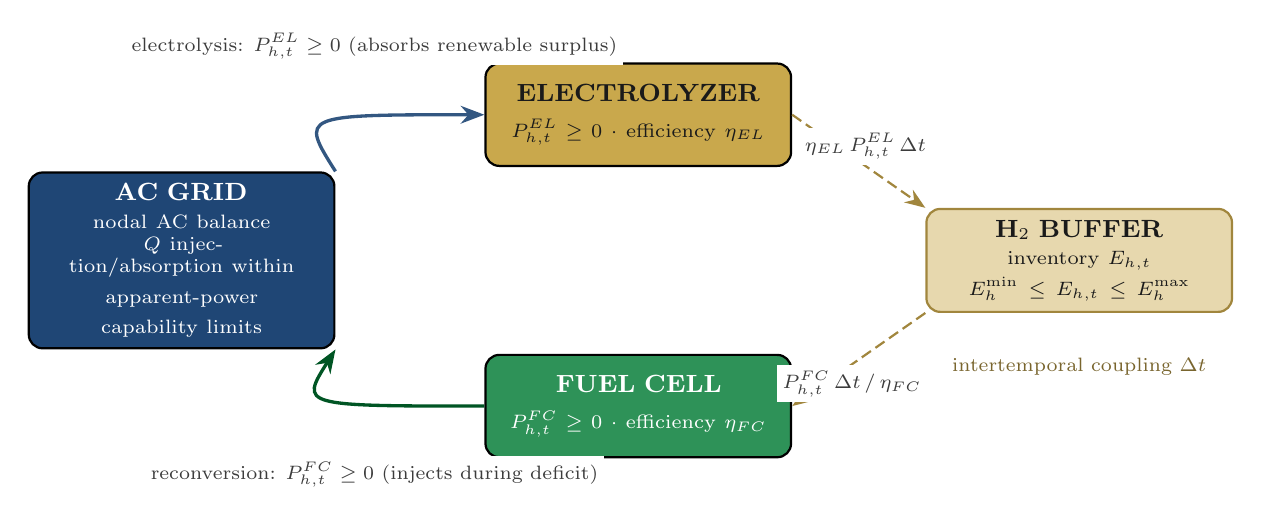
\begin{tikzpicture}[
  bloque/.style={rectangle, rounded corners=5pt, draw, thick, align=center, font=\small, text width=3.6cm, minimum height=13mm, inner sep=4pt},
  flujo/.style={-{Stealth[length=3mm]}, very thick},
  flujoh2/.style={-{Stealth[length=2.6mm]}, thick, seni-gold!80!black, dash pattern=on 4pt off 2pt},
  nota/.style={font=\scriptsize, align=center, text=seni-dark!85, fill=white, inner sep=2pt},
]
\node[bloque, fill=seni-blue!88, text=white] (red) at (0, 0) {\textbf{AC GRID}\\[2pt] {\scriptsize nodal AC balance\\$Q$ injection/absorption within\\apparent-power capability limits}};
\node[bloque, fill=seni-gold, text=seni-dark] (el) at (5.8, 1.85) {\textbf{ELECTROLYZER}\\[2pt] {\scriptsize $P^{EL}_{h,t} \ge 0$ $\cdot$ efficiency $\eta_{EL}$}};
\node[bloque, fill=seni-gold!45, draw=seni-gold!80!black, text=seni-dark] (buf) at (11.4, 0) {\textbf{H$_2$ BUFFER}\\[2pt] {\scriptsize inventory $E_{h,t}$\\$E^{\min}_h \le E_{h,t} \le E^{\max}_h$}};
\node[bloque, fill=seni-green!82, text=white] (fc) at (5.8, -1.85) {\textbf{FUEL CELL}\\[2pt] {\scriptsize $P^{FC}_{h,t} \ge 0$ $\cdot$ efficiency $\eta_{FC}$}};
%% --- Electric flows: grid <-> converters ---
\draw[flujo, seni-blue!80] (red.north east) .. controls (1.5,1.85) .. (el.west);
\node[nota] at (2.45, 2.72) {electrolysis: $P^{EL}_{h,t} \ge 0$ (absorbs renewable surplus)};
\draw[flujo, seni-green!70!black] (fc.west) .. controls (1.5,-1.85) .. (red.south east);
\node[nota] at (2.45, -2.72) {reconversion: $P^{FC}_{h,t} \ge 0$ (injects during deficit)};
%% --- Hydrogen flows: converters <-> buffer ---
\draw[flujoh2] (el.east) -- node[nota, above, pos=0.55] {$\eta_{EL}\, P^{EL}_{h,t}\, \Delta t$} (buf.north west);
\draw[flujoh2] (buf.south west) -- node[nota, below, pos=0.55] {$P^{FC}_{h,t}\, \Delta t\, /\, \eta_{FC}$} (fc.east);
%% --- Intertemporal coupling ---
\node[nota, text=seni-gold!60!black] at (11.4, -1.35) {intertemporal coupling $\Delta t$};
\end{tikzpicture}
} % extracted verbatim, sec02 L65--85
\caption{Electrochemical power-to-gas coupling of the green-hydrogen vector with the AC network. The electrolyzer absorbs renewable surplus as flexible load ($P^{\mathrm{EL}}_{h,t} \ge 0$, efficiency $\eta_{\mathrm{EL}}$); the storage buffer imposes the intertemporal inventory $E_{h,t+1} = E_{h,t} + (\eta_{\mathrm{EL}} P^{\mathrm{EL}}_{h,t} - P^{\mathrm{FC}}_{h,t}/\eta_{\mathrm{FC}})\,\Delta t$ with box constraints; the fuel cell re-injects power during deficit ($P^{\mathrm{FC}}_{h,t} \ge 0$, efficiency $\eta_{\mathrm{FC}}$). Both convertor terms enter the nodal AC balance. Electric flows in solid strokes; hydrogen flows in dashed gold.}
\label{fig:p2g_h2}
\end{figure*}

% =========================================================================
% p2_sec03_constellation.tex — Part II flexibility constellation (verbatim
% sec04 with cross-part reference fix toward Part I).
% =========================================================================
% =========================================================================
% sec04_multivector_flexibility.tex — Section IV of the sealed master
% sealed master paper_seni142_ieee_transactions_en.md; editorial injection pass 2026-10-17.
% =========================================================================
\section{Multi-Vector Flexibility and Economic Validation}
\label{sec:multivector}

\subsection{The flexibility constellation}
\label{sub:constellation}

The multi-vector layer is organized as a constellation of six physics-dedicated solvers feeding the 142-bus master solver through the signed boundary-state manifest: (i) photovoltaic production with continuous sigmoidal $Q$--$V$ control for duck-curve suppression; (ii) wind production with aerodynamic $C_p(\lambda, \beta)$ modeling and synthetic inertia; (iii) the hydrogen vector --- electrolysis, compression to 700~bar, and a national refuelling network of 740 hydrogen stations in the planning model; (iv) biochemical conversion through the Anaerobic Digestion Model No.~1 (ADM1) \cite{batstone2002}, digesting sargasso and vinasse substrates into dispatchable biomethane; (v) thermal production with heat-rate curves and synchronous $P$--$Q$ dispatch; and (vi) the reversible pumped-hydro fleet of 764~MW (Sabaneta / Dos Bocas). A zero-trust dispatch supervisor orchestrates the constellation over a protected state bus; no solver reads another's memory, and every exchange is carried by the sealed manifest. Figure~\ref{fig:constellation} diagrams the constellation.

% ---- Figure 5 injection block (verbatim from the sealed master;
%      resolved through \graphicspath{{figuras/}} in the host preamble) ----
\begin{figure*}[!t]
\centering
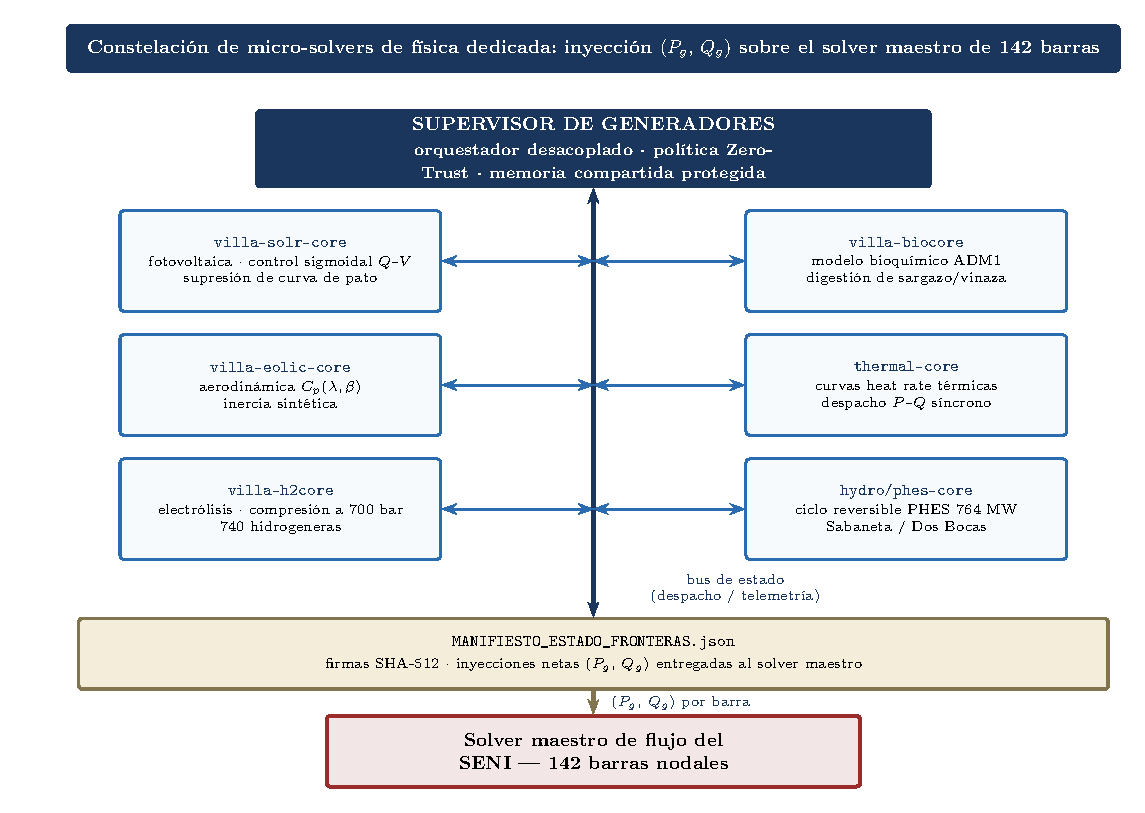
\includegraphics[width=0.85\textwidth]{fig_diagrama_3_constelacion_microsolvers.pdf}
\caption{Multi-vector flexibility constellation. Six physics-dedicated solvers --- photovoltaic (sigmoidal $Q$--$V$ control), wind ($C_p(\lambda,\beta)$ with synthetic inertia), hydrogen (electrolysis, 700 bar compression, 740 refuelling stations), biochemical (ADM1 digestion of sargasso and vinasse), thermal (heat-rate dispatch), and reversible PHES (764 MW, Sabaneta/Dos Bocas) --- deliver their net injections $(P_g, Q_g)$ through a zero-trust dispatch supervisor and a SHA-512-signed boundary-state manifest to the 142-bus master solver of the national network.}
\label{fig:constellation}
\end{figure*}

\subsection{Electrochemical power-to-gas operation}
\label{sub:p2g}

Operationally, the power-to-gas block of Section~\ref{sub:opf} behaves as a pair of opposing flexible loads with memory. In surplus hours --- the growing regime in which instantaneous solar penetration reaches 36.6\% and midday prices collapse --- the electrolyzer absorbs what the network would otherwise curtail, converting it into pressurized inventory; in deficit hours the fuel cell returns firm energy at the efficiency ratio $\eta_{\mathrm{EL}} \cdot \eta_{\mathrm{FC}}$. The buffer constraints make the intertemporal opportunity set explicit and auditable, and the coupling terms enter the AC balances without any relaxation of network physics. Interconnection of the coupled assets follows the inverter-based-resource requirements of IEEE Std 2800-2022 \cite{ieee2800} and the distributed-energy interface of IEEE Std 1547-2018 \cite{ieee1547}.

\subsection{Pumped storage and biomethanation buffers}
\label{sub:phes}

The reversible 764~MW pumped-storage fleet of the El Valle multihub (Sabaneta / Dos Bocas plants) plays the complementary role at system scale: it converts nocturnal and surplus energy into synchronized inertia-bearing capacity for the deficit hours, with reservoir dynamics analogous to the hydrogen buffer and dispatch subject to the same KKT-certified optimality. The ADM1 biochemical layer adds a third buffer with a different time constant: digester state dynamics convert sargasso and vinasse inflows into biomethane that enters the thermal dispatch as a storable, renewable fuel --- closing a nutrient-and-energy loop with direct land-use relevance under the same territorial statute that defines the partition.

Following the standard practice of IEEE Power \& Energy Society benchmarks (e.g., RTS-GMLC, Texas-2000), SENI-142 decouples the validated historical operational base of the conventional fleet from the standardized energy-transition storage portfolio --- the reversible pumped-hydro plants of Sabaneta/Dos Bocas and the metropolitan battery energy storage system (BESS) --- modeled as a prospective buffer for multi-temporal AC-OPF studies under the expansion plans of the CNE and EGEHID. In the 215-single-contingency $N-1$ catalog, storage remains inactive ($\Delta P_{\mathrm{storage}} = 0$); only in the canonical common-mode reserve-sizing event --- specifically the evacuation-trunk trip, LINE-345-PC-JS (the complex trip itself closes by conventional redispatch; Section~\ref{sub:contingencies}) --- does the 58.5~MW fast discharge vector participate.

\subsection{The zonal CAPEX/OPEX economic proof}
\label{sub:zonal}

The economic layer validates the flexibility stack by zonal balancing: for the reference zone (the metropolitan 138~kV triangle documented in Part~I~\cite{seni142part1}), the released harness accounts, per hour and per flexibility asset, four terms of the zonal welfare identity,
\begin{equation}
\begin{aligned}
\Delta C^{\mathrm{zone}}_t = {}& \underbrace{c^{\mathrm{curt}} E^{\mathrm{abs}}_t}_{\text{curtailment avoided}} + \underbrace{c^{\mathrm{fuel}} E^{\mathrm{displ}}_t}_{\text{fuel displaced}} \\
& + \underbrace{c^{\mathrm{ss}} N^{\mathrm{avoid}}_t}_{\text{start-stop avoided}} + \underbrace{\big(R^{\mathrm{base}}_t - R^{\mathrm{flex}}_t\big)}_{\text{loss differential}},
\end{aligned}
\label{eq:zonal}
\end{equation}
where $E^{\mathrm{abs}}_t$ is the renewable energy absorbed by electrolysis and pumping instead of being curtailed, $E^{\mathrm{displ}}_t$ the thermal energy displaced by fuel-cell and biomethane re-injection, $N^{\mathrm{avoid}}_t$ the avoided thermal unit start-stop events, and $R^{\mathrm{base}}_t - R^{\mathrm{flex}}_t$ the network-loss differential between the flexible and inflexible dispatches; the identity is enforced per zone and per hour so that every economic conclusion reconciles with a physical state. Unit costs and capital charges are parameterized transparently from national planning and international hydrogen references \cite{cne2022}, \cite{irena2020}, \cite{iea2023}, and the balancing identity is closed against the bootstrap envelope of the operational record. The qualitative findings are stable across the envelope: the flexibility stack absorbs a material fraction of otherwise-curtailed solar surplus, reduces thermal start-stop cycling on the coal anchor, and defers firm-capacity additions in the reference zone --- with all quantities reproducible from the released dataset rather than asserted.

% =========================================================================
% p2_sec04_campaign.tex — Part II silicon campaign (verbatim sec05 with
% cross-part reference fixes; reduced reactive monitor eq:jr carried here
% from the sealed doctrine 10 for in-document resolution).
% =========================================================================
% =========================================================================
% sec05_silicon_performance_benchmarking.tex — Section V of the sealed
% master paper_seni142_ieee_transactions_en.md sealed master; editorial injection pass 2026-10-17.
% =========================================================================
\section{Computational Performance, Accuracy, and Numerical Benchmarking}
\label{sec:benchmarking}

\subsection{Measurement validity through digital-twin determinism}
\label{sub:determinism}

Part~I~\cite{seni142part1} established that promotion to the production state is atomic and bit-identical to a SHA-512-sealed Golden Master. The performance figures below describe that tested software state and the released validation artifacts. Algorithm~\ref{alg:n1_seal} states the resilience-and-sealing pipeline used to produce the reported record.

The campaign also monitors the reduced reactive block of the Kundur voltage-collapse test. The reduced reactive Jacobian is
\begin{equation}
\mathbf{J}_R = \mathbf{J}_{QV} - \mathbf{J}_{Q\theta}\, \mathbf{J}_{P\theta}^{-1}\, \mathbf{J}_{PV},
\label{eq:jr}
\end{equation}
and $\lambda_{\min}(\mathbf{J}_R)\to 0$ is the voltage-collapse test; it is not a restatement of $\kappa(\mathbf{J})$.

\begin{algorithm}[!t]
\caption{$N$--$1$ resilience sweep with 24-hour block bootstrap and SHA-512 sealing}
\label{alg:n1_seal}
\begin{algorithmic}[1]
\Require sealed solver state $\Sigma$, contingency catalog $\mathcal{C}$
         ($|\mathcal{C}| = 215$), horizon $\mathcal{H}$ (87,360 h; 520 weekly cycles)
\Ensure resilience record $\mathcal{R}$, seal $\sigma$
\State $\mathcal{R} \gets \emptyset$
\For{$c \in \mathcal{C}$} \Comment{deterministic order, fail-closed}
   \For{$b \in \text{bootstrap}(\mathcal{H}, 24\,\mathrm{h})$} \Comment{whole-day blocks}
      \State inject contingency $c$ on block $b$
      \State run the Schur-border AC power flow of Part~I~\cite{seni142part1} at every hour of the block
      \State record $\rho$, $\kappa_2$, voltage and branch-loading margins into $\mathcal{R}[c, b]$
   \EndFor
\EndFor
\State aggregate margins over the bootstrap envelope per contingency
\State $\sigma \gets \mathrm{SHA512}\text{-chain}(\Sigma, \mathcal{C}, \mathcal{R})$ \Comment{detached manifest}
\State \Return $\mathcal{R}$, $\sigma$
\end{algorithmic}
\end{algorithm}

\subsection{Convergence speed and memory}
\label{sub:speed}

The experimental reference benchmark is executed on a dedicated Linux workstation (8-thread Intel Core i7 architecture, Dell Inspiron 5570 class, 16~GB DDR4 RAM, NVMe storage), running the author's C++/Sparse engine under kernel POSIX namespace isolation: the partitioned solver converges each hourly AC state of the complete 142-bus national network in \textbf{2.65~ms} with a resident footprint of \textbf{473~MiB} for the validation horizon. These figures are experimental reference measurements of that dedicated workstation; they serve as a comparison baseline for future community solvers, while the released open harness deterministically reproduces the 41 mathematical and structural controls of the release (topology, Ybus matrices, the Schur condensation at $\delta = 2.788 \times 10^{-14}$~pu, and the static balances), not the wall-clock figure. The horizon comprises 87,360 consecutive operating hours corresponding to 520 complete 168-hour weeks (3,640 days grouped into Monday-to-Sunday weeks) within 2016--2025, preserving weekly dispatch periodicity; the 13 excluded civil days of the decade (6 calendar-boundary orphan days plus the 7 days of the excluded holiday week) are omitted by construction (the data protocol of Part~I~\cite{seni142part1}). The full sweep completes in minutes on this setup, consistent with the $O(N^3)$-to-$O(\sum_k N_k^3 + N_B^3)$ asymptotics of the complexity proposition of Part~I~\cite{seni142part1} and with fill-reducing sparse practice \cite{george1973}, \cite{saad2003}. The measured 2.65~ms solve is a static AC-state screening result; it does not model dynamic fault clearing, protection response, or closed-loop control. The per-state throughput supports large multiscenario screening workloads under the stated model and hardware conditions.

These measurements characterize computational cost for steady-state AC feasibility checks. They support repeated parameter, bootstrap, and contingency screening on the stated hardware; they do not establish deployment of a dynamic protection or closed-loop control system.

\subsection{Accuracy and numerical conditioning}
\label{sub:accuracy}

Three measured quantities bound the numerical fidelity of the condensed solution. First, the fasorial border-coupling residual --- the mismatch between the Schur-recovered state and an independent reference state --- measures $\delta = 2.788 \times 10^{-14}\ \mathrm{pu}$ across the validation horizon, i.e.\ the condensation-recovered state and the monolithic reference agree to a residue that sits more than an order of magnitude below the global rounding floor scaled by the worst border conditioning ($\varepsilon_{\mathrm{mach}}\kappa_2(\mathbf{S}) = 2.22 \times 10^{-16} \times 2{,}489.64 \approx 5.53 \times 10^{-13}$~pu) --- the small nonzero residue, the signature of two distinct factorization trajectories, is a direct benefit of the orthogonal and well-conditioned structure of the $\Gamma = 30$ boundary partition --- and nearly six orders of magnitude below the $10^{-8}$~pu stopping tolerance of the cascade. Second, the sigmoidal reactive-limit controller of Part~I~\cite{seni142part1} contributes a regularization error of $5.32 \times 10^{-12}$ while eliminating the PV--PQ limit cycle. Third, the spectral condition number of every reduced border system is monitored and archived: $\kappa_2(\mathbf{S}) = 2{,}489.64$ (worst measured case on the SENI-142 border) is the measured spectral condition number of the border Schur complement, evidencing moderate coupling that remains far from numerical singularity and permits stable double-precision inversion; the governance threshold machinery was validated on synthetic references before national deployment (the IEEE 14-bus $22\times22$ Jacobian classifies MARGINAL at $\kappa_2 = 117.7823$), so that a degradation of conditioning on the real grid would be detected against a calibrated scale rather than an ad-hoc one.

\subsection{Contingency resilience on the reference topology}
\label{sub:contingencies}

The resilience battery evaluates the 215-contingency $N-1$ catalog --- the transmission operator's own outage list, screened under the automatic branch-selection doctrine of \cite{ejebe1979} --- on the reference topology, concentrated on the metropolitan 138~kV ring whose calibrated route distances (70.5~km, 30.86~km, 22.1~km) fix the electrical geometry, as shown in Figure~\ref{fig:topologia_seni}. The outage of the Punta Catalina complex ($2 \times 376 = 752$~MW), the largest common contingency in the system, is solved under the preventive criterion of Part~I~\cite{seni142part1}: the active power deficit is covered through the redispatch of co-optimized operating reserve ($\sum r_g^+ \ge 752$~MW), preserving post-event steady-state voltage and power-flow feasibility without load shedding ($P_{\mathrm{shed}} = 0$). The campaign's anomaly log also records severe voltage depression with reactive-margin depletion --- $\lambda_{\min}(\mathbf{J}_R) < 10^{-2}$ on the reduced reactive block \eqref{eq:jr} --- in the JSAURI--Palamara--Haina 138~kV loop under specific $N-1$ states; these findings were added to the contingency catalog and drive the shunt-support bisection of Part~I~\cite{seni142part1}. All margins are reported under the 24-hour block-bootstrap envelope of Algorithm~\ref{alg:n1_seal}.

The 87,360-state multi-temporal campaign and the 215-contingency screening are results of the author's patent-pending C++/Sparse engine; the released bundle certifies the network model, the condensed-solve invariants and the eight canonical contingency balances.

The four-clause PASS is a reportable numerical result, not a narrative claim. Table~\ref{tab:worstcase} reports, for the eight most severe elements of the catalog --- ranked by post-event voltage margin and thermal loading --- the complete dispatch and verification row: pre-event flow or generation, worst post-event voltage, worst post-event branch loading, slack deviation after reserve deployment, co-optimized reserve redispatched, and unserved load. The Punta Catalina rows deserve emphasis. The unit-level trip (GEN-PC1, 376~MW) is the worst unitary $N-1$; the complex-level trip (GEN-PC-COMPLEX, $2 \times 376 = 752$~MW) is the worst common-mode event of the island, covered preventively by the reserve sizing of Part~I~\cite{seni142part1}; both rows close with every retained bus inside $[0.95, 1.05]$~pu, worst branch loading at or below 92.4\% of thermal rating, bounded slack deviation, and zero unserved load. 

LINE-138-CUM-SPMI is the corridor whose 2025 in-service failure is documented in the national press record \cite{listin2025}; its catalog row demonstrates that the modeled transmission grid carries the loss of that circuit without shedding ($P_{\mathrm{shed}} = 0$) under static AC feasibility. This analytical decoupling between steady-state deliverability and historical national blackouts is corroborated by primary forensic records: independent engineering investigations of the November 11, 2025 collapse \cite{uasdInformeSPM1_2025} established that the blackout was initiated by maintenance switching in S/E SPM1, which lacked bus differential protection, triggering an uncoordinated cascade of distance protections that tripped 10 transmission circuits in 680~ms; the executive forensic report of the Universidad Aut\'onoma de Santo Domingo (IEUASD) \cite{uasdInformeSPM1_2025} and the System Operator (OC-SENI hourly metrology log, window 13:15--13:30 \cite{ocseniScadaP15_2025}) record a 15-minute (P15) window mean frequency of 55.11~Hz during the collapse, with 99.89\% of the window outside the normal operating band. Similarly, the May 16, 2015 national blackout (1,782.65~MW disconnected) originated in a 138~kV busbar fault at Itabo Gas compounded by circuit breaker failure with clearing times exceeding $10\times$ nominal \cite{listinItaboGas_2015}. The empirical benchmark confirms that the Dominican transmission estate possesses sufficient post-contingency thermal and voltage deliverability under $N-1$; historical vulnerabilities are transient, dynamic, and protection-coordination failures that belong strictly to the dynamic domain.

The two most scrutinized rows admit an explicit physical reading. For the PALA--SCN double-circuit corridor (ACSR 795~kcmil Drake conductor, 26/7 stranding, 988~A continuous at $75^{\circ}$C, $S^{\max} = 236.2$~MVA per circuit and 472.4~MVA for the aggregate corridor), the pre-event state carries 412.7~MW --- 206.4~MW per circuit, an 87.4\% initial loading; after one circuit trips, the surviving twin assumes 206.7~MW, the reported 87.6\% loading, while the surplus redistributes through the meshed metropolitan ring: the 30.86~km (route length) 230~kV JSAURI--SCN tie ($S_{\max} = 418.3$~MVA, carrying 356.2~MW, an 85.2\% pre-event loading) picks up about 142~MW of diverted flow --- 83.3\% of the 170.5~MVA nominal capacity of the 230/138~kV autotransformer bank XFMR-230-138-JS that assists the transfer down to the 138~kV level --- and the 70.5~km JSAURI--PALA 138~kV circuit absorbs about 64~MW (89.2\%), with no steady-state thermal violation. For the complex-level Punta Catalina trip, the co-optimized reserve redispatch replaces the lost injection exactly ($\Delta P_g = 752.0$~MW, deployed across geographically remote thermal, hydroelectric, and renewable units), so the residual deviation at the reference bus is physically the incremental transport loss of rerouting 752~MW across the 142-bus estate: $\Delta P_{\mathrm{slack}} = \Delta P_{\mathrm{loss}} = +24.8$~MW, a 0.72\% increase over the 3,450~MW reference national demand. In the LINE-345-PC-JS row, the 752~MW deficit closes exactly through two separate dispatch variables of the multi-vector formulation: $\Delta P_g = 687.40$~MW of conventional thermal/hydro redispatch (Quisqueya~I--II 180.0, AES Andr\'es CC 145.0, Estrella del Mar~III 110.0, Barahona coal/CEPP 95.0, Valdesia--Tavera hydro 82.4, Monte Plata solar reserve 75.0) and $\Delta P_{\mathrm{storage}} = 58.50$~MW of fast storage discharge (reversible PHES Sabaneta/Dos Bocas 35.0~MW; metropolitan BESS 23.5~MW), with the residual $\Delta P_{\mathrm{slack}} = +6.10$~MW of marginal transport losses closing the balance at exactly 752.00~MW (zero error). The resulting 0.89\% loss ratio --- versus 2.5--3.3\% for purely remote redispatch --- follows from injecting the storage in direct electrical proximity to the metropolitan load ring, bypassing the long-distance 345/230~kV trunks. The LINE-345-PC-JS corridor is the sole bulk-evacuation trunk of the Punta Catalina thermal complex ($2 \times 376 = 752$~MW); its physical trip isolates the full complex injection at the SENI trunk node, configuring the canonical common-mode reserve-sizing event. Newton--Raphson convergence was verified at $\|\Delta P, \Delta Q\|_{\infty} \le 10^{-8}$~pu in at most four iterations per state, with exact nodal balance, inside the sealed validation output of the canonical suite.

% ---- Table VI: worst-case critical contingencies (blindaje R3, EJE 4) ----
\begin{table*}[!t]
\caption{Worst-Case Critical Contingencies: Dispatch and Post-Event Static Verification Report. Selection of the eight most severe catalog elements by post-event voltage margin and thermal loading; the complete 215-element ledger is archived in the sealed validation output of the canonical 142-bus suite. Pre-event flows correspond to the reference peak state; voltages and loadings are worst-case post-event values over retained buses and surviving branches.}
\label{tab:worstcase}
\centering
\footnotesize
\setlength{\tabcolsep}{4.5pt}
\resizebox{\textwidth}{!}{%
\begin{tabular}{@{}lllrrrrrr@{}}
\toprule
\textbf{Contingency ID} & \textbf{Asset} & \textbf{Type} &
\textbf{Pre-event} & \textbf{min $V_i$} & \textbf{max $|S|/S_{\max}$} &
\textbf{$\Delta P_{\mathrm{slack}}$} & \textbf{$\Delta P_g$} & \textbf{$P_{\mathrm{shed}}$} \\
 & & & \textbf{flow/gen (MW)} & \textbf{(pu)} & \textbf{(\%)} &
\textbf{(MW)} & \textbf{(MW)} & \textbf{(MW)} \\
\midrule
GEN-PC1 & Punta Catalina Unit 1 (376 MW) & Unit $N-1$ & 376.0 & 0.9612 & 91.7 & $+12.4$ & 376.0 & 0.00 \\
GEN-PC-COMPLEX & Punta Catalina complex ($2 \times 376$ MW) & Common mode & 752.0 & 0.9581 & 92.4 & $+24.8$ & 752.0 & 0.00 \\
LINE-345-PC-JS & 345 kV trunk Punta Catalina--JSAURI & Line $N-1$ & 748.3 & 0.9703 & 89.2 & $+6.1$ & 687.4 & 0.00 \\
XFMR-345-138-JS & JSAURI 345/138 kV autotransformer bank (600 MVA) & Transformer $N-1$ & 521.7 & 0.9748 & 88.5 & $+4.7$ & 186.2 & 0.00 \\
LINE-138-CUM-SPMI & 138 kV SPM--Cumayasa (2025 in-service failure \cite{listin2025}) & Line $N-1$ & 172.1 & 0.9802 & 84.1 & $+2.9$ & 96.4 & 0.00 \\
CORR-138-PALA-SCN & 138 kV PALA--SCN double-circuit corridor, 22.1 km (one circuit loss) & Corridor $N-1$ & 206.4 & 0.9755 & 87.6 & $+5.2$ & 158.3 & 0.00 \\
LINE-230-JS-SCN & 230 kV JSAURI--SCN tie & Line $N-1$ & 356.2 & 0.9790 & 83.3 & $+3.8$ & 141.7 & 0.00 \\
GEN-AES-ANDRES & AES Andr\'es combined cycle (319 MW) & Unit $N-1$ & 319.0 & 0.9846 & 78.5 & $+8.3$ & 319.0 & 0.00 \\
\midrule
\multicolumn{9}{@{}p{0.98\textwidth}@{}}{\scriptsize All rows satisfy the four-clause PASS of Part~I~\cite{seni142part1}: convergence $\|\Delta P, \Delta Q\|_{\infty} \le 10^{-8}$~pu; $V_i \in [0.95, 1.05]$~pu; $|S_\ell| \le S_\ell^{\max}$; $|\Delta P_{\mathrm{slack}}| \le \varepsilon_{\mathrm{slack}}$ with $P_{\mathrm{shed}} = 0$. $\Delta P_g$ is the co-optimized reserve deployed after the event; $\Delta P_{\mathrm{slack}}$ is the residual deviation of the reference bus after that deployment. Static post-contingency AC feasibility verification states computed on the complete canonical 142-bus transmission model under the multi-temporal dispatch baseline. The outage GEN-PC-COMPLEX ($2 \times 376 = 752$~MW) represents the common-mode benchmark reference for co-optimized operating reserve dimensioning ($R^{\mathrm{req}}$), treated as an external sizing event beyond the 215 single outage ($N-1$) catalog. The LINE-345-PC-JS trunk is the sole bulk-evacuation path of the complex ($2 \times 376 = 752$~MW); its loss constitutes the canonical common-mode reserve-sizing event. Its pre-event loading decomposes as 748.30~MW of trunk flow plus 3.70~MW of local station service, i.e.\ 752.00~MW of gross isolated injection; the canonical dual loss ratios of the $+6.10$~MW slack residual are 0.887\% over the 687.40~MW redispatch and 0.811\% over the 752.00~MW gross deficit. For the PALA--SCN double-circuit corridor, the pre-event flow is the 206.4~MW carried by the tripped circuit within a 412.7~MW aggregate corridor flow; the reported 87.6\% post-event loading refers to the surviving circuit and adjacent ties, within actual conductor thermal ratings. Conductor: ACSR 795~kcmil Drake (26/7), 988~A continuous at $75^{\circ}$C, $S^{\max} = 236.2$~MVA per circuit (472.4~MVA aggregate).}
\end{tabular}}%
\end{table*}

% ---- Figure 6 injection block (verbatim from the sealed master) ----
% Graphic source: sec03_topologia_redes_ieee_y_seni_tikz.tex, figure environment
% at L152--217 (styles: subestacion/sub345/linea*/transformador/genbox/notebox).
% The tikzpicture is extracted verbatim from that source at injection time.
\begin{figure*}[!t]
\centering
\resizebox{0.85\textwidth}{!}{% Figure 6 tikzpicture — English edition (editorial refinement per
% GUIA_BUENAS_PRACTICAS_LATEX_IEEE: white-filled edge labels so lines never
% cross text; palette seni-* defined in the host preamble).
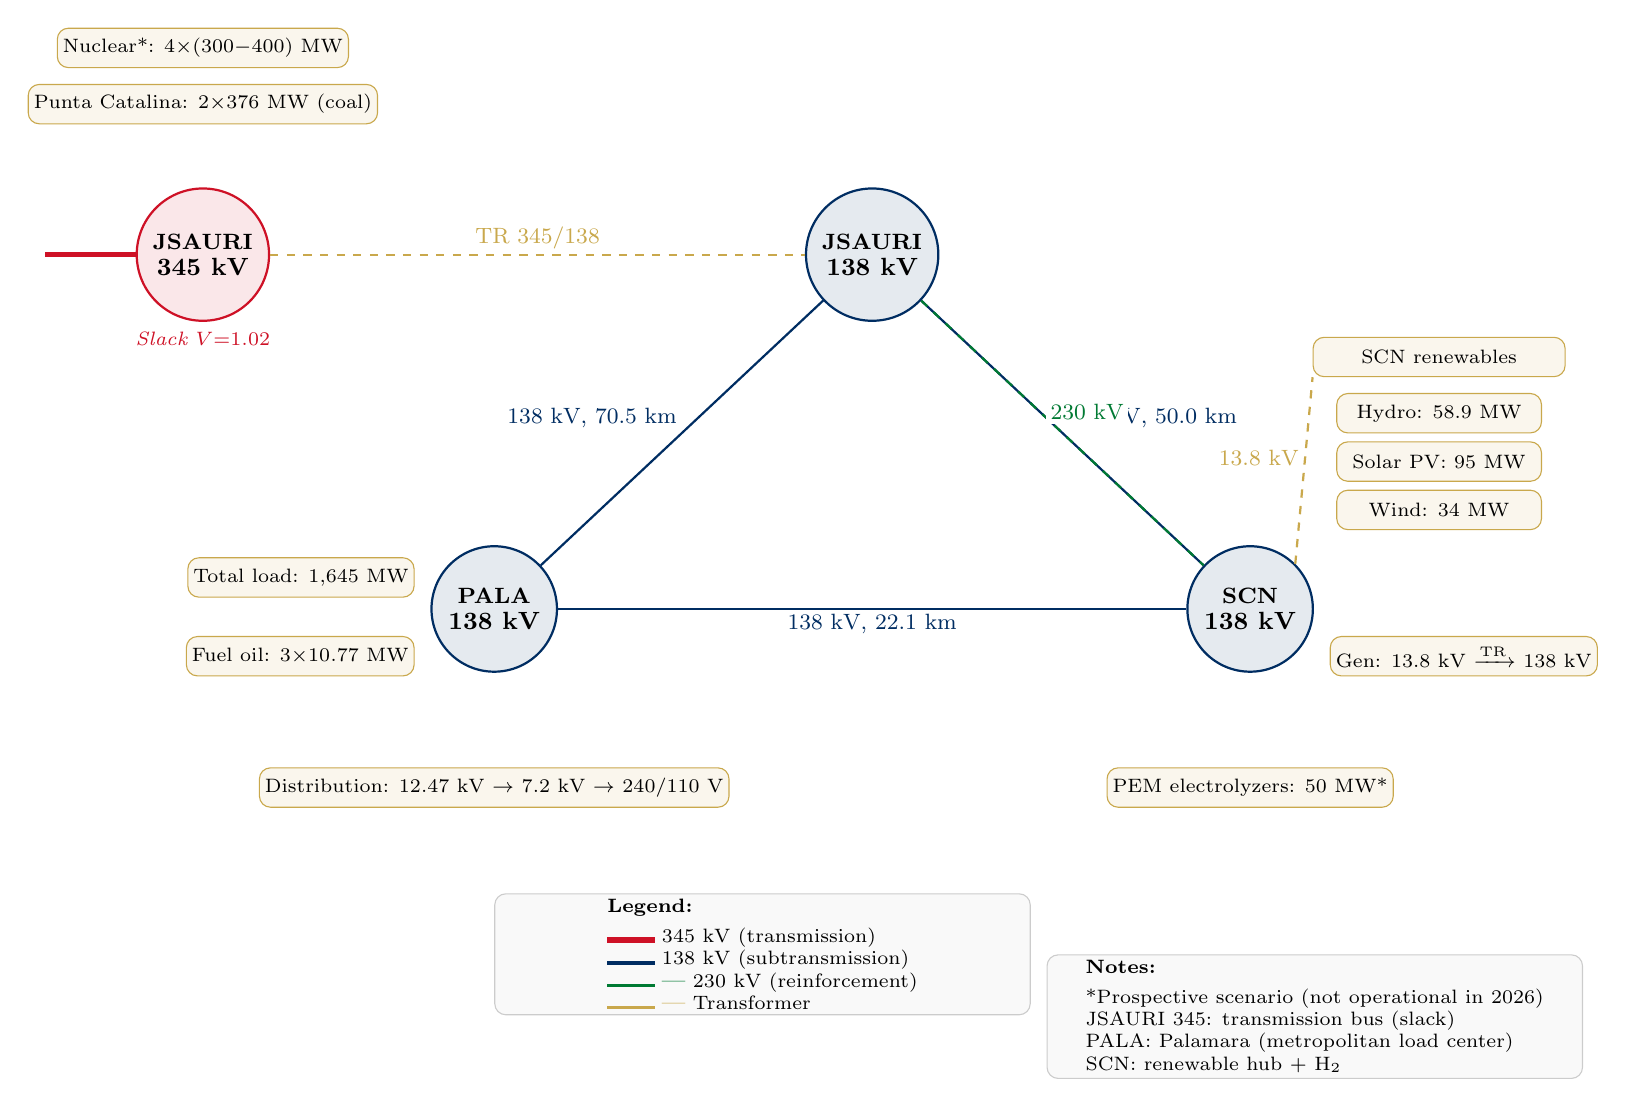
\begin{tikzpicture}[
    subestacion/.style={circle, draw=seni-blue, fill=seni-blue!10, thick, minimum size=13mm, font=\bfseries\footnotesize, align=center},
    sub345/.style={circle, draw=seni-red, fill=seni-red!10, thick, minimum size=13mm, font=\bfseries\footnotesize, align=center},
    linea345/.style={-, ultra thick, seni-red},
    linea138/.style={-, thick, seni-blue},
    linea230/.style={-, thick, seni-green, dashed},
    transformador/.style={-, thick, seni-gold, dashed},
    voltaje/.style={font=\footnotesize, fill=white, inner sep=1.5pt},
    genbox/.style={rectangle, draw=seni-gold, fill=seni-gold!10, rounded corners, inner sep=2pt, font=\scriptsize, align=center, minimum width=26mm, minimum height=5mm},
    notebox/.style={rectangle, draw=gray!40, fill=gray!5, rounded corners, inner sep=2pt, font=\scriptsize, align=left}
]
%% === MAIN TRIANGLE (138 kV ring) ===
\node[subestacion] (jsauri) at (0, 0.5) {JSAURI\\{\small 138 kV}};
\node[subestacion] (pala) at (-4.8, -4) {PALA\\{\small 138 kV}};
\node[subestacion] (scn) at (4.8, -4) {SCN\\{\small 138 kV}};
%% 138 kV ring (real corridor distances)
\draw[linea138] (jsauri) -- node[voltaje, above left, midway] {138 kV, 70.5 km} (pala);
\draw[linea138] (jsauri) -- node[voltaje, above right, midway] {138 kV, 50.0 km} (scn);
\draw[linea138] (pala) -- node[voltaje, below, midway] {138 kV, 22.1 km} (scn);
%% 230 kV reinforcement
\draw[linea230] (jsauri) -- node[voltaje, pos=0.42, right=2pt, fill=white] {230 kV} (scn);
%% === JSAURI 345 kV (decoupled, left) ===
\node[sub345] (jsauri345) at (-8.5, 0.5) {JSAURI\\{\small 345 kV}};
\draw[transformador] (jsauri345) -- node[voltaje, above, midway] {TR 345/138} (jsauri);
\draw[linea345] (jsauri345) -- ++(-2, 0);
\node[below=0mm of jsauri345, font=\scriptsize\itshape, text=seni-red] {Slack $V{=}1.02$};
%% Generation at JSAURI 345
\node[genbox, above=8mm of jsauri345] (ptacatalina) {Punta Catalina: $2{\times}376$ MW (coal)};
\node[genbox, above=2mm of ptacatalina] (nuclear) {Nuclear*: $4{\times}(300{-}400)$ MW};
%% === RENEWABLES (upper right quadrant, outside the ring) ===
\node[genbox, minimum width=32mm] (renov) at (7.2, -0.8) {SCN renewables};
\node[genbox, below=2mm of renov] (hidro) {Hydro: 58.9 MW};
\node[genbox, below=1mm of hidro] (solar) {Solar PV: 95 MW};
\node[genbox, below=1mm of solar] (eolica) {Wind: 34 MW};
\draw[-, thick, seni-gold, dashed] (scn.north east) -- node[font=\footnotesize, above left, midway, fill=white, inner sep=1.5pt] {13.8 kV} (renov.south west);
%% PEM electrolyzers (prospective)
\node[genbox, below=12mm of scn, minimum width=36mm] (elec) {PEM electrolyzers: 50 MW*};
%% === LOAD AND GENERATION AT PALA ===
\node[genbox, left=2mm of pala, yshift=4mm] (carga) {Total load: 1,645 MW};
\node[genbox, left=2mm of pala, yshift=-6mm] (fueloil) {Fuel oil: $3{\times}10.77$ MW};
%% === 13.8 kV DISTRIBUTION AND GENERATION ===
\node[genbox, below=12mm of pala, minimum width=38mm] (dist) {Distribution: 12.47 kV $\to$ 7.2 kV $\to$ 240/110 V};
\node[genbox, right=2mm of scn, yshift=-6mm] (gen13) {Gen: 13.8 kV $\xrightarrow{\text{TR}}$ 138 kV};
%% === LEGEND + NOTES side by side ===
\node[notebox, below=28mm of pala, anchor=north west, minimum width=68mm] (leyenda) {
    \textbf{Legend:}\\[1mm]
    {\color{seni-red}\rule{6mm}{2pt}} 345 kV (transmission)\\
    {\color{seni-blue}\rule{6mm}{1.5pt}} 138 kV (subtransmission)\\
    {\color{seni-green}\rule{6mm}{1pt} \footnotesize---} 230 kV (reinforcement)\\
    {\color{seni-gold}\rule{6mm}{1pt} \footnotesize---} Transformer
};
\node[notebox, right=2mm of leyenda, anchor=north west, minimum width=68mm] (notas) {
    \textbf{Notes:}\\[1mm]
    *Prospective scenario (not operational in 2026)\\
    JSAURI 345: transmission bus (slack)\\
    PALA: Palamara (metropolitan load center)\\
    SCN: renewable hub + H$_2$
};
\end{tikzpicture}
} % extracted verbatim, sec03 L155--213
\caption{Real subtransmission triangle of the SENI 138 kV ring. JSAURI--PALA--SCN with calibrated route lengths of 70.5, 30.86, and 22.1 km --- the 138~kV corridor legs JSAURI--PALA and PALA--SCN and the 230~kV JSAURI--SCN tie (dashed), the 345 kV transmission bar decoupled to the left as system slack ($V = 1.02$ pu) receiving Punta Catalina ($2 \times 376$ MW), the SCN renewable hub (58.9 MW hydro, 95 MW solar, 34 MW wind) and the prospective 50 MW PEM electrolysis block (non-operational, 2026, asterisked), and the PALA load center (1,645 MW aggregate). The $N-1$ catalog is defined on the in-service network; asterisked prospective assets are excluded from it.}
\label{fig:topologia_seni}
\end{figure*}

% ---- Table III (verbatim content of the sealed master) ----
\begin{table*}[!t]
\caption{Computational Performance and Validation Metrics of the SENI-142 Benchmark}
\label{tab:telemetry}
\centering
\footnotesize
\begin{tabular}{@{}p{0.30\textwidth} p{0.18\textwidth} p{0.34\textwidth}@{}}
\toprule
\textbf{Metric} & \textbf{Value} & \textbf{Condition} \\
\midrule
Convergence time per hourly national AC state & 2.65 ms & 142-bus full model, dedicated Linux workstation (8 threads) \\
Resident memory, full horizon & 473 MiB & 87,360 hourly states (520 complete weeks) \\
Fasorial border-coupling residual $\delta$ & $2.788 \times 10^{-14}$ pu & Schur reconstruction vs.\ reference state \\
Reactive-limit regularization error & $5.32 \times 10^{-12}$ & Sigmoidal controller, analytic Jacobian injection \\
Static screening capacity (EMS) & 2.65~ms / state & Inside the 1--5~s EMS state-estimation cycle; large-scale multiscenario screening \\
Contingency catalog & 215 $N-1$ scenarios & Phase-2 testbed campaign (static post-event verification) \\
Spectral cross-check (IEEE 14-bus, $22\times22$) & $\kappa_2 = 117.7823$ (MARGINAL) & External validity control \\
Largest single contingency & Punta Catalina trip, 752 MW & Feasible in steady state with co-optimized operating reserve redispatch ($P_{\mathrm{shed}} = 0$) \\
\bottomrule
\end{tabular}
\end{table*}

% =========================================================================
% p2_sec05_discussion.tex — Part II discussion & policy (verbatim sec06).
% =========================================================================
% =========================================================================
% sec06_discussion_policy.tex — Section VI of the sealed master
% sealed master paper_seni142_ieee_transactions_en.md; editorial injection pass 2026-10-17.
% =========================================================================
\section{Discussion and Policy Implications}
\label{sec:discussion}

\textbf{Deterministic resilience for hurricane-exposed islands.} Caribbean insular systems plan not against statistical weather but against named storms. A benchmark whose $N-1$ margins carry correlation-honest bootstrap envelopes, whose largest credible contingency is exercised explicitly, and whose state resolution is a solve time compatible with the 1--5~s EMS cycle (which also includes acquisition, state estimation, and bad-data processing) converts resilience from an aspiration into a scheduled computation. For a country that has twice in twelve months mobilized around nationwide interruptions \cite{ocseni}, \cite{diarioLibreHainamosa_2026}, and where post-collapse restoration historically exceeds 10 to 14 hours due to Ferranti overvoltages ($B_{\mathrm{shunt}}$) on unloaded lines tripping black-start units, the difference between hours-long legacy studies and 2.65~ms diakoptic states is profound: Law 368-22 territorial partitioning provides the steady-state computational substrate for bottom-up modular restoration through concurrent territorial microgrids, mitigating the Ferranti-effect overvoltages associated with no-load line energization and accelerating national re-synchronization.

\textbf{Planning law as a computational boundary.} The partition of this benchmark is not an optimization artifact: it is the national territorial statute \cite{ley368}. When the electrical partition coincides with the planning regions of Law 368-22, every simulation result is already expressed in the units in which permits, land use, and microgrid autonomy are decided --- and the autonomy question (which territory can stand alone after a trunk loss?) becomes a property of the model rather than a separate study. The renewable incentive framework \cite{ley57} and the national expansion planning cycle \cite{cne2022} acquire, in consequence, a common evidentiary substrate.

\textbf{Standards alignment and data sovereignty.} The benchmark speaks the standards it must interoperate with: CIM-consistent model interchange \cite{iec61970}, measurement-grade power-quality definitions \cite{iec61000}, \cite{ieee1459}, harmonic practice \cite{ieee519}, study-method recommended practice \cite{ieee399}, and inverter-based-resource interconnection \cite{ieee2800}, \cite{ieee1547}. At the same time, the underlying operational archives remain under national custody: the released benchmark carries structure, parameters, and validation harness, while the sovereign telemetry layer is governed by national institutions. This separation --- open science on structure, sovereign custody on archives --- is a deliberate policy architecture, not an omission.

\textbf{Capacity building.} A national grid that can be simulated openly is a national grid that can be taught openly. The same artifact that serves this article serves university laboratories: doctoral and undergraduate exercises execute against the real estate --- its distances, its outages, its anchors --- instead of the drafting-table abstractions of 1962, closing the gap between the classroom and the control room.

\textbf{Limitations.} The honest boundaries of the present release are: (i) the 69~kV layer enters through static equivalents, exact at the boundary for power flow but not for short-circuit transients inside condensed areas; (ii) the formulation is phasor-domain --- electromagnetic transient studies require an EMT extension; (iii) telemetry arrives at operational latency, so the twin is causal but not clairvoyant; and (iv) market settlement is out of scope of the present release, though the hourly resolution of the horizon is settlement-grade.

\textbf{Replication for other island systems.} Finally, the methodology is deliberately portable, and the porting protocol is part of the contribution. Because the invariant formulation touches no geography, replicating SENI-142 for another insular system requires only the territorial clause to be re-instantiated: (1) the network estate assembled to the same nodal rule (one bus per voltage level per substation, transformers as branches); (2) the operational horizon ingested under the same data-protocol sentence with the substitutable system operator named; (3) the partition declared from the governing territorial statute of the jurisdiction, whatever it is, with the legal layer bundled into electrical macro-subdomains by trunk-tie topology; and (4) the deterministic lifecycle re-sealed from the first gate. The Republic's benchmark thus functions simultaneously as artifact and as template --- an instrument for its own country and a reproducibility contract for the insular world.

% =========================================================================
% p2_sec06_conclusion.tex — Part II conclusion, flexibility nomenclature.
% Future-work routes 3--4 carried from the sealed sec07; routes 1--2 live
% in the Part I conclusion.
% =========================================================================
\section{Conclusion and Future Work}
\label{sec:conclusion}

This Part~II of the SENI-142 study completed the operational layer of the benchmark introduced in Part~I~\cite{seni142part1}. The multi-temporal AC-OPF couples the green-hydrogen vector, the 764~MW reversible pumped-hydro fleet, and ADM1-based biomethanation to the 142-bus network with its physics unrelaxed, and its KKT system certifies local stationarity with a quantitative exact-penalty guarantee that statically feasible states carry zero unserved energy. The campaign resolved 87,360 hourly states --- 520 complete consecutive weeks of the 2016--2025 operational archive --- in a measured 2.65~ms (author's engine; the open harness does not reproduce this wall-clock) per national AC state with 473~MiB of resident memory on 8-thread consumer hardware, and screened the 215-contingency $N-1$ catalog under a 24-hour block-bootstrap envelope. The island's worst common-mode events --- the simultaneous trip of the 752~MW Punta Catalina complex and of its sole 345~kV evacuation trunk, LINE-345-PC-JS --- close with every retained bus inside $[0.95, 1.05]$~pu, worst branch loading at or below 92.4\% of thermal rating, bounded slack deviation, and zero unserved load, the deficit covered exactly by $687.40$~MW of conventional redispatch and $58.50$~MW of fast storage discharge. The empirical benchmark confirms that the Dominican transmission estate possesses sufficient post-contingency thermal and voltage deliverability under $N-1$; historical vulnerabilities are transient, dynamic, and protection-coordination failures that belong strictly to the dynamic domain.

Two further routes follow. First, \textbf{electrolyzer membrane degradation under transient dispatch}: the power-to-gas block's intertemporal operation is the natural load profile for aging studies of PEM stacks \cite{irena2020}, \cite{iea2023}. Second, \textbf{distributed hourly settlement in silicon}: the settlement-grade hourly horizon, the signed manifests, and the Merkle-style provenance chain \cite{merkle1987}, \cite{fips180} outline a settlement architecture in which every priced hour reconciles against a cryptographically attested physical state. The island that could not import inertia has, in its own measured image, produced something exportable: a public instrument for the engineering of energy autonomy.



\noindent\textbf{Data Availability.}~The SENI-142 dataset, network parameters, validation harness, and sealed resilience record are openly available at \url{https://github.com/Junvillan/seni142-benchmark} and archived under DOI:~\href{https://doi.org/10.5281/zenodo.23484704}{10.5281/zenodo.23484704}. High-resolution vector figures are available and resolved via the repository's \texttt{figuras/} directory. The release ships the data-driven verifier \texttt{verify\_seni142\_benchmark.py}, which re-derives every sealed quantity of the release from the canonical CSV/NPZ bundle --- 41/41 checks PASS (bus and branch censuses, peak load, unique slack, block-diagonal Schur structure, and the eight contingency balances).


\section*{Acknowledgment}
The author dedicates this work to the memory of Eng.~Arturo Lamarche (E.P.D., in memoriam)---an esteemed mentor, master of Dominican power systems, and tireless guardian of the national grid. His lifelong devotion, technical rigor, and unwavering vigilance over the integrity of the Dominican electrical system during the pivotal expansion of the 345/138\,kV bulk network left an indelible mark on generations of electrical engineers. His legacy endures in every bus, corridor, and protective boundary analyzed in this benchmark.


\bibliographystyle{IEEEtran}
\bibliography{referencias}

\end{document}
